\begin{frame}
	\frametitle{Inversion about average}
	\begin{tikzpicture}[
	expl/.style={draw=black, thick=2pt,fill=blue!20,rounded corners},
	arrow/.style={red!80!black,ultra thick,->,>=latex}]	
	\node[anchor=south west,inner sep=0] (image) at (0,0) {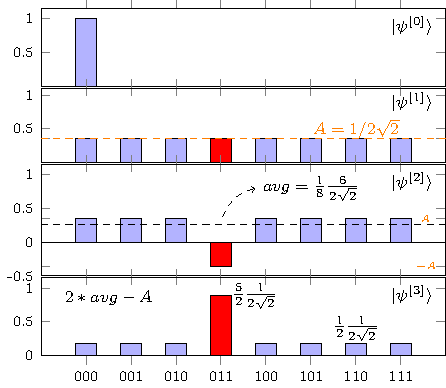
\includegraphics[width=0.5\textwidth]{figures/bar-graph/probs.pdf}};
	\begin{scope}[x={(image.south east)},y={(image.north west)}]
	%\draw[help lines,xstep=.1,ystep=.1] (0,0) grid (1,1);
	%\foreach \x in {0,1,...,9} { \node [anchor=north] at (\x/10,0) {0.\x}; }
	%\foreach \y in {0,1,...,9} { \node [anchor=east] at (0,\y/10) {0.\y}; }
	\node[expl](A) at (1.5,0.875) {\Large Initial state $\ket{\psi^{[0]}}$};
	\node[expl](B) at (1.5,0.65) {\Large Initialization $\ket{\psi^{[1]}}$};
	\node[expl](C) at (1.5,0.4) {\Large Sign flip $\ket{\psi^{[2]}}$};
	\node[expl](D) at (1.5,0.15) {\Large Inversion about average $\ket{\psi^{[3]}}$};
	
	\draw[arrow] (A.south) -- node [right]{Hadamard $H$} (B.north);
	\draw[arrow] (B.south) -- node [right]{Oracle $U_f$} (C.north);
	\draw[arrow] (C.south) -- node [right]{Difussion $U_d$} (D.north);
	\draw[thick,dashed] (0.01,0.0) rectangle (1.925,0.5);
	\draw[arrow] (D.north east) to[bend right] node [right]{$\frac{\pi}{4}\sqrt{n}$} (B.east);
	\end{scope}
	
	\end{tikzpicture}	
\end{frame}
\begin{frame}
	\frametitle{Inversion about the average}
	We find a method (unitary operator) to invert the amplitude about the average
	\pause
	\begin{equation*}
		\sum_{j\in\{0,1\}^{n}}\alpha_{j}\left.|j\right\rangle _{n}\stackrel{U_d}{\longrightarrow}\sum_{j\in\{0,1\}^{n}}\left(2\left(\sum_{k\in\{0,1\}^{n}}\frac{\alpha_{k}}{2^{n}}\right)-\alpha_{j}\right)\left.|j\right\rangle _{n},
	\end{equation*}
	where $\sum_{k\in\{0,1\}^{n}}\frac{\alpha_{k}}{2^{n}}$ is the average.
	\begin{exampleblock}{}
		\[\sum_{k\in\{0,1\}^{n}}\frac{\alpha_{k}}{2^{n}}=\frac{1}{2^3}\frac{6}{2\sqrt{2}}\]
	\end{exampleblock}
\end{frame}
\begin{frame}
	\frametitle{Inversion about the average}
	\begin{block}{\textit{Difussion operator}}
		\begin{eqnarray}
			U_{d}=\left(\begin{array}{cccc}
			\frac{2}{2^{n}} & \frac{2}{2^{n}} & \cdots & \frac{2}{2^{n}}\\
			\frac{2}{2^{n}} & \frac{2}{2^{n}} & \cdots & \frac{2}{2^{n}}\\
			\vdots & \vdots & \ddots & \vdots\\
			\frac{2}{2^{n}} & \frac{2}{2^{n}} & \cdots & \frac{2}{2^{n}}
			\end{array}\right)-I^{\otimes n}=\dots=-H^{\otimes n}DH^{\otimes n},
		\end{eqnarray}
		where $D=diag\left(-1,1,1,\cdots,1\right)$
	\end{block}
\end{frame}

\begin{frame}[fragile]{}
	\frametitle{Inversion about the average}
	\begin{exampleblock}{3-qubit example: Difussion operator in python}
		\vspace*{0.5cm}
		\begin{adjustbox}{max width=0.9\textwidth}
			\begin{python}
>>> import numpy as np
>>> H1 = 1/np.sqrt(2)*np.array([[1,1],[1, -1]]) # Hadamard operator 1 qubit
>>> H2 = np.kron(H1,H1) # Hadamard operator 2 qubit
>>> H3 = np.kron(H2,H1) # Hadamard operator 3 qubit

>>> D = np.eye(8) # Diagonal operator
>>> D[0,0] = -1

>>> Ud = -np.dot(np.dot(H3,D),H3) # Difussion operator
>>> psi_2 = 1/(2*np.sqrt(2))*np.array([1,1,1,-1,1,1,1,1]) # psi_2

>>> psi_3 = np.dot(Ud,psi_2)
>>> print(psi_3)
array([0.176 , 0.176 , 0.176 , 0.883, 0.176, 0.176, 0.176, 0.176])
			\end{python}
		\end{adjustbox}
	\end{exampleblock}

\end{frame}
\begin{frame}
	\frametitle{Inversion about the average}
	\begin{exampleblock}{3-qubit example: Difussion operator}
	\begin{eqnarray}
	\ket{\psi^{[3]}}&=&U_d\ket{\psi^{[2]}}\nonumber\\
	\ket{\psi^{[3]}} &=& -\frac{1}{8}\frac{1}{2\sqrt{2}}\begin{pmatrix*}[r]
	6 & -2 & -2 & -2 & -2 & -2 & -2 & -2\\
	-2 & 6 & -2 & -2 & -2 & -2 & -2 & -2\\
	-2 & -2 & 6 & -2 & -2 & -2 & -2 & -2\\
	-2 & -2 & -2 & 6 & -2 & -2 & -2 & -2\\
	-2 & -2 & -2 & -2 & 6 & -2 & -2 & -2\\
	-2 & -2 & -2 & -2 & -2 & 6 & -2 & -2\\
	-2 & -2 & -2 & -2 & -2 & -2 & 6 & -2\\
	-2 & -2 & -2 & -2 & -2 & -2 & -2 & 6
	\end{pmatrix*}
		\begin{pmatrix*}[r]
		1\\
		1\\
		1\\
		-1\\
		1\\
		1\\
		1\\
		1
		\end{pmatrix*}=\frac{1}{4\sqrt{2}}
		\left(
		\begin{tabular}{c}
		1\\
		1\\
		1\\
		5\\
		1\\
		1\\
		1\\
		1
		\end{tabular}
		\right)\nonumber
	\end{eqnarray}
	\end{exampleblock}
\end{frame}